\chapter{Overview of Absorption Spectroscopy}\label{ch:overview}

Spectroscopy is a field of science dedicated to using the knowledge of how
electromagnetic radiation interacts with matter. The fact that matter absorbs,
emits, refracts, and deflects energy allows us to investigate the properties
of a substance non-invasively, allowing a wealth of information to be acquired
without altering the matter being probed. The information that can be gleaned
from such experiments include the chirality of a molecule, the energy levels
of an atom's electronic structure, and the concentration of various chemicals
in any type of solution, to name only a few.

This chapter will discuss a variety of absorption spectroscopy techniques.
First, a discussion of the theory behind absorption spectroscopy will be
presented. Afterward an in depth look at different absorption spectroscopy
techniques used to increase sensitivity and applicability is performed.



\section{Theory behind Absorption Spectroscopy}\label{sec:abs_theory}

Absorption spectroscopy is founded on a simple principle: if matter absorbs
light, then it is possible to detect this energy transfer via the law of the
conservation of energy. One of the simplest ways to measure an absorption
event is to count the number of photons that went into a substance in question
and how many photons came out the other side. In this way it can be determined
how much energy was absorbed by the matter in the substance, assuming no light
is lost to scattering or other processes. The amount of light absorbed is
correlated to the concentration of the absorbing material in the path of the
light, and the absorption amount is unique to the absorber and its current
state. The information about photon absorption can then be used to understand
not only the concentration of the absorber but its electronic structure as
well.



\subsection{Beer-Lambert Law}\label{subsec:beer}

Mathematically, the problem of determining the concentration of an absorber
based on the light lost in a material is relatively simple. By measuring the
amount of light of a particular wavelength $\lambda$ entering a material, with
intensity $I_0$, and the amount of light exiting $I$, a relationship of the
intensities to each other can be made to determine how much light was lost due
to absorption \cite{Hollas:2004uh}.

\begin{align*}
  \left(\frac{I}{I_0}\right)_\lambda = e^{-\alpha(\lambda)l}
\end{align*}

In the equation above, $\alpha$ is known as the \emph{absorption coefficient}
(with units of \icm), and is unique to the absorber and the wavelength used as
the probe. $l$ is the path length that the light travels through the absorbing
material. The intensity loss due to absorption is caused by an electron in
the absorber being elevated to a higher energy state. Since electrons can be
elevated to a multitude of quantised energy states, it is important to choose
a wavelength that corresponds to one of these electronic transitions.

Taking the logarithm of both sides leads to a value known as the absorbance $A$

\begin{align}
  A(\lambda)=-\ln\left(\frac{I}{I_0}\right)_\lambda = \alpha(\lambda)l\label{eq:beer}
\end{align}


\begin{wrapfigure}{o}{\marginspace}
\begin{center}
  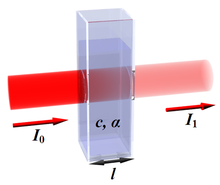
\includegraphics[width=\marginspace]{figures/beer.png}
\end{center}
\emph{\footnotesize{Light passing through a sample cavity is attenuated by the absorbers within the solution. Courtesy Wikipedia.}}
\label{fig:microtiter}
\end{wrapfigure}

This is known as the Beer Lambert law. The law relates the loss of light in a
material to the concentration of absorbers inside that material based on the
amount of light passing through the absorber and the properties of the absorber
itself.  While this version of the  law is formulated using a natural logarithm, it is also common to see the law in a base ten format \cite{Hollas:2004uh}.

The Beer-Lambert law can also be used for multiple absorbers in a single material by simply adding the absorption coefficients of all of the absorbers together.

\begin{align*}
  A(\lambda) = l\sum\alpha(\lambda)_i
\end{align*}

While the Beer-Lambert law is simplistic, it falls prey to some simple sources of interference, including the following \cite{Skoog:1994wg}.
\begin{itemize}
  \item Little tolerance to other light loss pathways such as scattering.
  \item Optical saturation limits, where the absorbers cannot accept any more light due to already being in an excited state.
  \item Requires a homogeneous mixture of the absorbers.
  \item A collimated light sources to allow the path length to be constant.
\end{itemize}

\marginpar{Pulse oximeters can be used together with other technologies to
acquire physiological parameters across the entire body: see the Esoma project.
\url{http://www.rdodesigns.com}}

Despite these limitations, the Beer-Lambert law has found many uses in modern
analytical devices. One of the most familiar devices is a pulse oximeter, which
measures blood oxygenation levels in a patients blood. This is done by passing
light across the patient's index finger to see how much light was lost to
oxygenated and deoxygenated blood. The concentrations of these two types of
blood can then be used to derive the total body blood oxygenation levels to a
high degree of accuracy \cite{Wukitsch:1987tb}.



\subsection{Electronic Transitions}\label{subsec:elec_trans}

\marginpar{In this section will be talking about atoms but the concepts apply to molecules as well}

Knowing how to measure concentration using absorption measurements is useful,
but with broadband light sources it is possible to measure absorption events
due to several different electronic transitions within an absorber. This
information can then be used for a better understanding of the absorber in
question, and allow properties such as fluorescence lifetimes to be measured
from absorption events \cite{Werts:2002fs}.

In addition to experimentally probing an absorber to determine its electronic
structure, it is possible to theoretically guess both the energy required for
an electronic transition and where it will take place. This is often done
through Hartree-Fock approximations to determine the energy required for an
electronic transition \cite{Szabo:1996tu}, and Judd-Ofelt theory to guess the
absorption strength at that transition \cite{Judd:1962uq}.



\section{Complications in Absorption Spectroscopy}\label{sec:comp_abs}

While absorption spectroscopy can be applied to a variety of materials, there
are several phenomenon that reduce the potential applicability of the
technique. Two of these phenomena -- spectral line broadening and scattering
losses -- are discussed below.



\subsection{Line Broadening}\label{subsec:line_broad}

Under theoretical conditions, with perfectly still particles, absorption lines
would be exceptionally thin due to the fact that only certain quantised energy
packets would create an excited condition. In reality, absorption lines are
quite broad, on the order of a few nanometers in liquid \cite{Hollas:2004uh}.
This broadening occurs due primarily to two factors: the Doppler effect
and collision based broadening (also known as Lorentzian or pressure based
broadening) \cite{Olivero:1977ul}.

Doppler based broadening is the Doppler effect applied to moving particles.
A particle at rest will see a incoming photon of light having a certain
frequency. If this particle is instead moving away from the photon, the
frequency of the light will appear to the particle as a lower frequency than
when the particle was standing still, as the distance between the crests and
troughs of the wave is greater in the particles inertial frame. Conversely,
if the particle is moving towards the photon, the photon will appear to have
a higher frequency than when the particle was standing still. The particle
in question will still absorb at the same quantised energy, but now photons
with greater and lesser energy than the transition will appear to have the
correct energy, broadening the range of wavelengths that the particle absorbs
\cite{Fox:2006uy}.

Collision based broadening leads to a similar effect of a broadening of
acceptable photon energies, but through a pressure pathway. As particles in
the solution collide into each other, they acquire some energy that puts them
in a state higher than their ground energetic state. As such, less energy is
required by the photon to cause an absorption event, leading to the absorption
of lower energy photons \cite{Ngo:2012jk}.

Both of these effects alter the absorption peaks in a spectra of an
aqueous absorber, leading to very broad absorption peaks. These broadening
effects lead to difficulty in the analysis of the acquired spectrum in two
different ways.

First, if two absorption peaks are too close together, they will appear as
one combined absorption peak. This causes a loss of information, as it is
impossible in most cases to calculate the absorption due to one transition
versus its nearby neighbor \cite{Fowles:1975wg}. This type of loss of
information does not often occur for electronic transitions in a molecule, as
the accepted electronic transitions are spaced out energetically due to the
higher energy required to jump to a higher molecular orbital. The collision of
absorption signals does become a problem when multiple absorbers are present
in a solution, often leading to signals that cannot be decoupled from one
another.

The second difficulty broadening causes in analysis is the understanding of
the hyperfine structure of certain transitions. When an electron is excited to
a higher energy state, it can often be excited into a multiplet of rotational
and vibrational energy states \cite{Levine:2008uh}. On top of this, many
degenerate energy states can exist for one transition, which will only be seen
if an external electric or magnetic field causes the fields to split (via
the Stark effect) \cite{Condon:1951wd}. These different states are separated
from each other by minute differences in energy, making the transitions
unobservable in liquid solutions.



\subsection{Scattering Losses}\label{subsec:scattering}

\begin{wrapfigure}{o}{\marginspace}
\begin{center}
  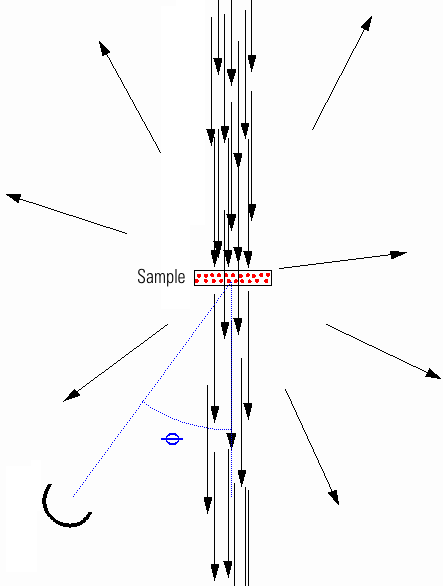
\includegraphics[width=\marginspace]{figures/scatter.png}
\end{center}
\emph{\footnotesize{Scattering of photons from molecules in a sample. Courtesy Wikipedia}}
\end{wrapfigure}

In addition to broadening schemes, liquid absorption measurements fall victim
to the fact that Beer-Lambert type experiments cannot differentiate between
light lost due to scattering versus due to absorption.  In gas phase
measurements, scattering is often not a concern due to the density of objects
on which scattering could occur. However, with the higher probability of a
photon being scattered in liquids, the assumption that scattering plays a minor
role in light loss is no longer valid. This leads to higher baseline error and
requires higher light intensities to be pumped into the absorbing medium, since
much of the  light will be lost just by trying to traversing the cavity.

The loss of light due to scattering also restricts the types of solutions that
can be observed. If a solution is turbid it may be difficult to find a powerful
enough light source that can push enough photons through the sample to detect
any light after the sample medium. Similarly, a solution that becomes turbid
during a measurement through either chemical reactions or colloidally will be
an impractical candidate for absorption measurements, as the loss of light due
to scattering changes over the time of the measurements. This turbidity problem
becomes especially pronounced in experiments designed to determine reaction
kinematics, as the absorption measurements over time will not be comparable due
to the shifting noise caused by scattering.

\marginpar{While a change in the normal index of refraction does not alter
absorption effects, a change in the complex index of refraction does cause
changes in absorption events due to the imaginary term}

Light can also be lost due to changes in the index of refraction for the
solution. Many gas solutions are dilute enough that the index of refraction of
the medium does not change significantly between measurements and blanks. This
scenario is different in liquids, where the index of refraction can change
significantly depending on the solvent and even the concentration of the
solute. This change in the index of refraction does not alter the absorption
events themselves, but presents a difficulty when attempting to align an
optical system. In the simple case of a single pass absorption, this effect can
lead to a loss of signal due to divergent beams that is dependent on the
wavelength, leading to a nonlinear error in the observed absorption spectrum.
In multipass systems, the misalignment of an optical cavity due to the change
in the index of refraction can preferentially support and discourage certain
modes, leading to a similar nonlinear error in an absorption spectrum. These
divergent beam problems can be mitigated by using a collimated source that
enters perpendicular to the cavity walls, negating the effects of the changes
in refraction. Unfortunately, in practice it is quite difficult to create a
perfect perpendicular alignment, and some error will always be present.

Even though broadening, scattering and changes in the index of refraction can
cause high and nonlinear errors to occur in absorption measurements, these
effects can be mitigated by a careful choice of the layout of the optical
system and the choice of the analyte. Experiments that measure clear solutions
with minimal changes in index of refraction are good candidates for absorption
spectroscopy, given that the experimenter does not require an understanding of
the hyperfine structure of the absorber in question.



\section{Broadband Absorption Spectroscopy}\label{sec:broad_abs}

The ideas gleaned from the Beer-Lambert law are dependent on wavelength of
light used to probe a material. As such, Beer-Lambert law is often used with a
single monochromatic light source and a simple photodiode as a detector.
However, there are many spectroscopic analyses that are not only concerned with
the absorption signal at a peak wavelength but in the shape of the transition
itself. Some applications require several absorption signatures to be measured
from a single sample. For these systems, absorption signals from a range of
wavelengths is required. Luckily, there are several methods that allow
experimenters to acquire absorption measurements at several wavelengths, both
sequentially and simultaneously.



\subsection{Tunable Diode Lasers}\label{subsec:tdl}

\begin{wrapfigure}{o}{\marginspace}
\begin{center}
\includegraphics[width=\marginspace]{figures/diode_laser.pdf}
\end{center}
\emph{\footnotesize{A simple laser diode, where the red ellipse represents the emission of light. Courtesy Wikipedia}}
\end{wrapfigure}

One common method for acquiring broadband signals is to use a light source
known as a \acf{TDL}. \ac{TDL} sources are diode lasers that are tunable
through either current or temperature \cite{May:1998ue}. Since temperature is
difficult to control, current is varied to sweep the frequency of the laser
light. This variation technique is used in \ac{TDLAS}, where the laser is
tuned to a particular frequency, an absorption measurement is taken, and then
this process repeats.

An advantage of \ac{TDLAS} over some of the other broadband techniques is that
the resolution of the instrument is dictated by the laser line width, which
provides sub nanometer resolution \cite{Berden:2009wk}. As a corollary, this
technique can use a simple photodiode or \ac{PMT} to acquire the intensity of
the laser light, instead of using a grating to disperse the light across a
detector.

\marginpar{A good discussion of wavelength modulation spectroscopy in the form
of an aircraft hygrometer can be found in \cite{May:1993tu}.}

Even though this method is simple to implement and cost effective, it suffers
from two major drawbacks. The first is that the broadband acquisition is done
sequentially, which creates an acquisition time versus resolution and spectral
range trade off to consider. \ac{TDLAS} also suffers from a problem inherent
to standard single pass absorption techniques, which is that the instrument
must detect a potentially small intensity change on top of a large background
signal. However, this second intensity problem can be mitigated through the use
either \ac{WMS} \cite{Reid:1981vq} or \ac{FMS}.



\subsection{LEDs}\label{subsec:led}

Another light source that has interesting potentials for broadband absorption
spectroscopy are \acp{LED}. \acp{LED} can provide light at a broad range of
frequencies and at high output intensities. \acp{LED} can even come in white,
infrared and ultraviolet variants, which can be used directly in absorption
spectroscopy. Best of all, these sources are extremely cheap to produce, making
\acp{LED} attractive sources for use in compact, inexpensive and portable
equipment.

Unfortunately \acp{LED} are quite difficult to use for absorption
spectroscopy.  \acp{LED} are incoherent sources, and as such it can be
difficult to couple the light from an \ac{LED} into a
cavity \cite{Seetohul:2009du,Islam:2007ea}. Even if light is successfully
coupled into the cavity containing absorber molecules, the amount of light
lost attempting to create a collimated beam often leads to minuscule fractions
of the light reach the detector.


\begin{wrapfigure}{o}{\marginspace}
\begin{center}
\includegraphics[width=\marginspace]{figures/led.pdf}
\end{center}
\emph{\footnotesize{A diagram of an \ac{LED}, courtesy Wikipedia.}}
\end{wrapfigure}

An additional complication from \acp{LED} is that once the broadband light
arrives at a photodetector the light must be separated into its constituent
wavelengths to acquire the broadband signal.  Two problems occur from this. If
one uses a spectrophotometer with a adjustable slit and moving diffraction
grating, then the signal acquired on a photodetector must be done
sequentially.  This increases the acquisition time, and suffers from reduced
spectral resolution when compared with a \ac{TDLAS} experiment due to the
limiting factor of the resolution being the diffraction grating. One can
mitigate the acquisition time conundrum by using a line detector instead of a
single photodetector, but this carries with it a second problem: the
acquisition, while happening simultaneously across several wavelengths, is
often more difficult to align and can lead to a lower spectral resolution as the line detectors elements have finite size and spacing.



\subsection{Supercontinuum Lasers}\label{subsec:super}

Supercontinuum laser light sources combine the advantage of a broadband source
with a tightly collimated beam and high output powers. This makes alignment
much simpler than in the case of an \ac{LED} with the added benefit of low
power loss while coupling into a absorbing medium.


\begin{wrapfigure}{o}{\marginspace}
\begin{center}
  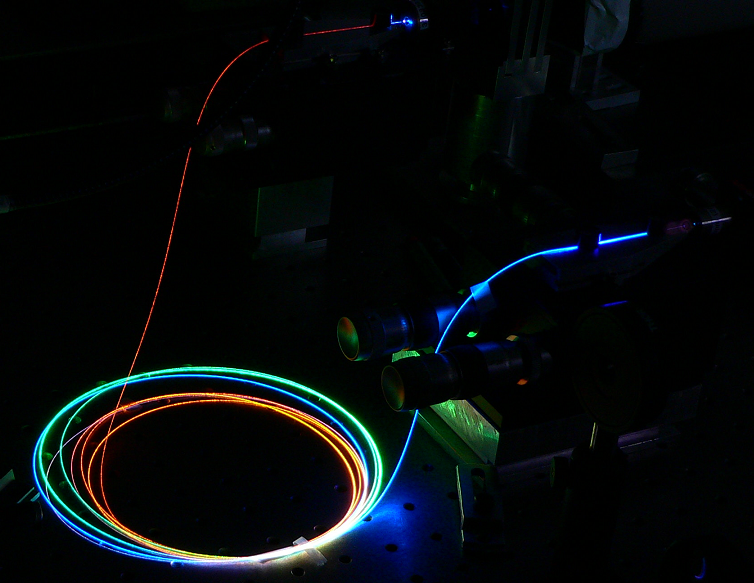
\includegraphics[width=\marginspace]{figures/supercontinuum.png}
\end{center}
\emph{\footnotesize{a Nd:YAG laser pulse being transformed into a supercontinuum by injecting the pulse into a photonic crystal fibre. Courtesy Wikipedia.}}
\end{wrapfigure}

While supercontinuum sources build on the advantages of \acp{LED}, they
introduce problems of their own. The most practical problem is the cost of
supercontinuum sources, which can cost upwards of \pounds40,000 at the time of
writing. Secondly, supercontinuum sources are prone to intensity fluctuations
over time and wavelength, and as such introduce higher error in an absorption
measurement.  Finally, these sources are not robust like \acp{LED} or
\acp{TDL}, and therefore cannot be taken outside of the laboratory.



\section{Multipass Techniques}\label{sec:multipass}

Besides acquiring broadband signals, it is also desirable to increase the
resolution of detectable concentrations and the lower limits of detection.
According to the Beer-Lambert law \eqref{eq:beer}, the simplest way to increase
the detection resolution is to increase the path length of the cavity. However,
as increasing the length of the sample cavity is often impractical due to
constraints of space or limitations of the absorbing molecules, it is common to
see optical designs that pass over the same sample several times. This is known
as a multiple pass technique. Two major versions of this technique are outlined
below.



\subsection{Multipass Cells}\label{subsec:herriott}


\begin{wrapfigure}{o}{\marginspace}
\begin{center}
  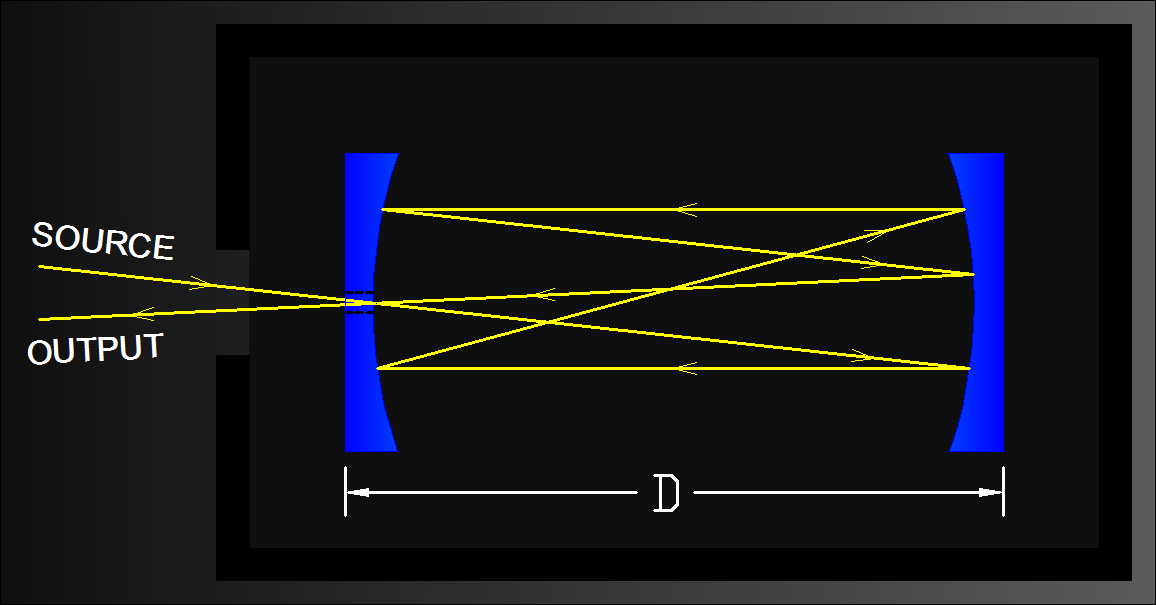
\includegraphics[width=\marginspace]{figures/herriott.png}
\end{center}
\emph{\footnotesize{A Herriott cell, shoring the path of light within the cell. Courtesy Wikipedia.}}
\end{wrapfigure}

One simple way to traverse a sample multiple times is to build a cavity with
two mirrors on either end that reflect the light back and forth through the
sample. It is possible to find mirrors that allow light to enter through a hole
in one mirror, bounce around a few times inside the cavity, and then exit
through a hole in the second mirror. These cavities are known as Herriott
cells, and they provide a simple and convenient way to increase the path
length \cite{Engel:2007va}. In the resulting measurement, the effective path
length is the distance across the sample multiplied by the number of passes,
making it possible to increase the resolution by a couple orders of magnitude.

These cells, while providing increased resolution, can be difficult to align.
In addition, Herriott cells can be misaligned once in place by accumulation of
particulates on the mirror surfaces.



\subsection{Optical Cavities}\label{subsec:cavity}


\begin{wrapfigure}{o}{\marginspace}
\begin{center}
  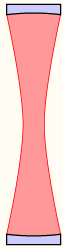
\includegraphics[height=100pt]{figures/cavity.png}
\end{center}
\emph{\footnotesize{An optical cavity and the light propagation inside using plano-convex mirrors. Courtesy Wikipedia.}}
\end{wrapfigure}

A similar approach to  Herriott cells is to use an optical cavity akin to a
laser cavity, except where both mirrors are only partially reflective. In such
a cavity, light leaks in through the first mirror, traverses across the sample
\emph{along the same path every pass} as the light bounces between the mirrors,
and then exits through the second mirror \cite{Berden:2009wk}. This method has an advantage over
Herriott cells in that the increase in the path length can be several orders of
magnitude higher if high reflectivity mirrors are used. For example, for
mirrors of reflectivity $R=0.999$, the increase in the path length will be
$(1-R)^{-1} = 1000$, which is a higher gain than most Herriott cells can
achieve.

Unfortunately these cavities are also difficult to align, as the input beam
must be perpendicular to the axis of the cavity. In addition, this method
requires a higher initial input intensity as a significant amount of light is
reflected when attempting to enter the cavity. Optical cavities introduce an
error due to the change in reflectivity of the mirrors based on wavelength that
must be measured and accounted for in the absorption spectrum. Finally, this
method can be more expensive than other multipass techniques, as high quality,
high reflectivity mirrors are expensive.

\marginpar{The mirror reflectivity curves depend on the alignment of the cavity
as well as the mirror surfaces. As such, it is not possible to use mirror
transmission curves provided by a manufacturer \cite{Berden:2009wk}.}



\section*{Chapter Review}

It is clear that absorption spectroscopy, based on the Beer-Lambert law
\eqref{eq:beer}, can be utilised to provide valuable information about a
material non-invasively. While the standard single pass technique can and has
been used successfully in commercial devices like pulse oximeters, there is
still a desire to increase the resolution of such systems to acquire
information on unlikely electronic transitions or minute traces of absorbers.
Augmentations that increase the path length and wavelength range of the
measured spectra are commonly in use today, and prove a cornerstone to
sensitive analytical techniques. In the coming chapters these improvements to
single pass absorption spectroscopy will be put to use to detect trace
concentrations of chemicals such as rhoadmine 6G and to analyse absorption
signatures of aqueous europium ions.
